\graphicspath{{../images/ch4/}}	% Image directory


\chapter{Hybrid resistive-pulse optical detections in microfluidic systems}
\label{chap:rpim}

	

	\section{Background \& Theory}
		
		As we have seen, RP sensing is a method for determining the physical properties of particles by way of measuring the change in resistance of a conducting channel they create as they pass through it. RP's primary advantage is that it can be employed at many scales and in a diverse number of applications, and is especially useful at the nanoscale where the number of particle characterization techniques is limited---in particular, optical imaging is prohibited at this scale. To first order, the mechanism for the rp current pulses is straight forward: when the particle enters the channel, it occupies a volume that would otherwise be occupied by ions, decreasing the conductance, and increasing the total system resistance. According to this simple model, the resistive of the system is determined solely by the equation
		
		\begin{equation}\label{eq:resistance}
			R=\rho\int A^{-1}\left(x\right) dx,
		\end{equation}
		
		where $R$ is the system resistance, $A\left(x\right)$ is the annular cross-section of the channel at position $x$, and $\rho$ is the resistivity of the solution. In most RP set ups, the current is measured instead of the resistance, so Eq. \ref{eq:resistance} is usually inverted via Ohm's law to obtain the current: $\Delta I/I_{p}=\Delta R/R_{0}$, where $I$ is the measured current, and the subscripts $0$ and $p$ denote quantities when the channel is empty, and occupied, respectively. While Eq. \ref{eq:resistance} serves as a good approximation for the RP amplitude that may be accurate in some cases, it fails to take into account the electrodynamic boundary conditions present in the system, namely that the normal component of the electric field vanishes at the surface of the insulating layer, or $\vec{E}\cdot\hat{n}\left.\right\vert_{\mathrm{surface}}=0$. The effects of boundary conditions can have a large influence on the measured RP amplitude that is position and geometry dependent, and therefore, most importantly can affect measurement of the size of a particle from the resistive pulse amplitude. Therefore, significant efforts have been directed towards finding more accurate expressions for specific particle and channel geometries. For instance, Smythe calculated the expected RP amplitude for spheres passing along the axis of cylindrical channels, and arrived at the expression
		
		\begin{equation}\label{eq:spherecylinderRP}
			\frac{\Delta I}{I_{p}}=\frac{d^{3}}{LD^{2}}\left[1-0.8\left(\frac{d}{D}\right)^{-3}\right]^{-1},
		\end{equation}
		
		where $d$ and $D$ are the diameter of the particle and pore, respectively, and $L$ is the length of the channel. Equation \ref{eq:spherecylinderRP} is probably the single most useful equation for sizing particles in resistive pulse experiments, however due to the preceding arguments we know it is only an approximation. For instance, the equation does not consider particles that travel off-axis, and it also assumes a channel length that is far greater than the length of the particle to be sized. Furthermore, it is only accurate for cylindrical channels and spherical particles. Few real-world experimental RP systems hold to these sterile conditions. 
		
		The typical route taken in cases where Eq. \ref{eq:spherecylinderRP} cannot fully capture the experimental findings is to devise a model that relates the position of the particle, the particle's geometry, and the geometry of the channel to the expected RP amplitude. Then, based on the model, conclusions are drawn from the RP signal about the positioning and dynamics of the translocation. As a concrete example, Berge \emph{et al.} observed a positive correlation between the translocation times and the RP amplitudes of microbeads that were driven through their channels by an applied pressure. They argued that, due to the Poiseuille flow profile present in their channel, a larger translocation time correlated to an off-axis displacement. The correlation between translocation time and amplitude then suggested a correlation between off-axis displacement and increases RP amplitude, which they explained was due to the increased distortion of the electric field, which increases the total system resistance, when the channel drifted laterally from the channel axis. As another example of an RP system which invalidated the conditions of Eq. \ref{eq:spherecylinderRP}, Tsutsui \emph{et al.} performed RP experiments with spheres in low-aspect ratio pores and found a significant variance in the observed RP amplitudes that could not be explained by size variance in the population alone. They argued, therefore, that the combination of particle and channel geometry created a unique situation where the observed RP amplitudes were highly trajectory dependent, and they then devised a model to relate the trajectory to the RP amplitude.
		
		In both of the above examples, the one-dimensional RP data set is used to study the complex dynamics of particle translocations through pores. The authors' inferences could very well be accurate, but could easily be validated or clarified by simply observing the translocations while simultaneously recording the RP data. However, the difficulty in performing such an experiment is the physical scale at which they worked; at the nanoscale, only electron microscopy is viable due to the optical diffraction limit. In most cases, \textit{in situ} electron microscopy during an RP experiment is prohibitively difficult. However, because RP experiments are largely scale independent, one possible option is to scale the solution up to a size where optical diffraction is possible, and to perform simultaneous RP and optical measurements. Such experiments could be used to clarify the positional dependencies of the RP signal, and the results would generalize back down to the nanoscale.
		
		In order to resolve the positional dependencies of the RP amplitudes, we devised a microfluidic experimental and data analysis platform that allows simultaneous RP and IM measurements and analysis. The experimental system is based on a high-speed camera combined with an optical microcope which captures images of particles as they pass through a microfluidic channel while the ionic current is simultaneously recorded (described in greater detail in the following section). By tracking particles simultaneously in the two data streams, we are able to create a position-RP amplitude mapping for each particle. The mappings of many particles are combined to create a `resistance map' of the channel, a two-dimensional plot of the local resistance in the channel as measured by the instantaneous RP amplitude $\Delta I/I_{p}$, and which can address specific questions about the positional dependencies of the resistive pulses. Such questions include but are not limited to:
		
		\begin{itemize}
			\item At which axial position does the RP amplitude attain its maximum value?
			\item What is the effect of lateral displacement of a particle inside the channel on its resulting RP amplitude?
			\item How is the variance distributed in variable-width channels, such as channels having a central cavity?
		\end{itemize}

		
		
	\section{Experimental hardware and software}
	      
		\begin{figure}
			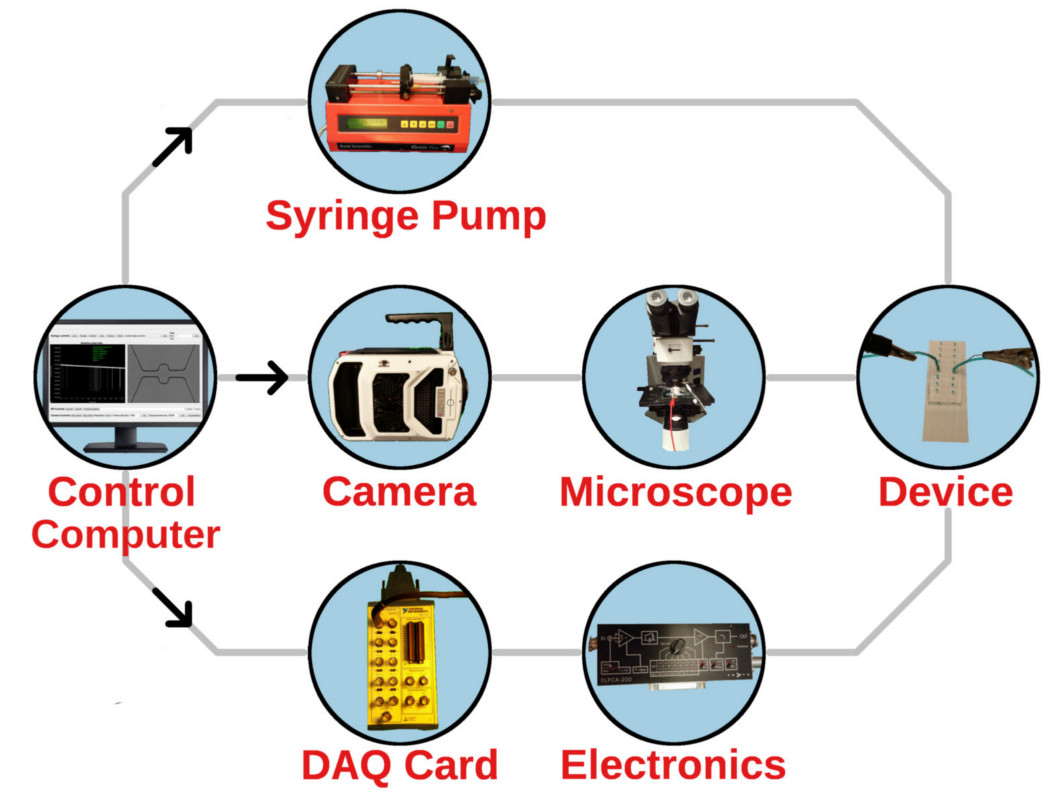
\includegraphics[width=\textwidth]{hardware.jpg}
			\caption{\textbf{Hardware set up for the hybrid RP-IM experiments.}}
			\label{fig:hardware}
		\end{figure}

	
		We devised a hybrid resistive pulse-optical imaging platform that is capable of resolving the spatial dependencies of the RP amplitude signals. The set up (Fig. \ref{fig:hardware}) consists of a high-speed camera combined with an optical microscope, all of the electronic equipment used to acquire the RP signal, a syringe pump to drive particle suspensions through the system, a planar microfluidic channel, and a central control computer used to run the experiment and record data.
		
		\begin{figure}
			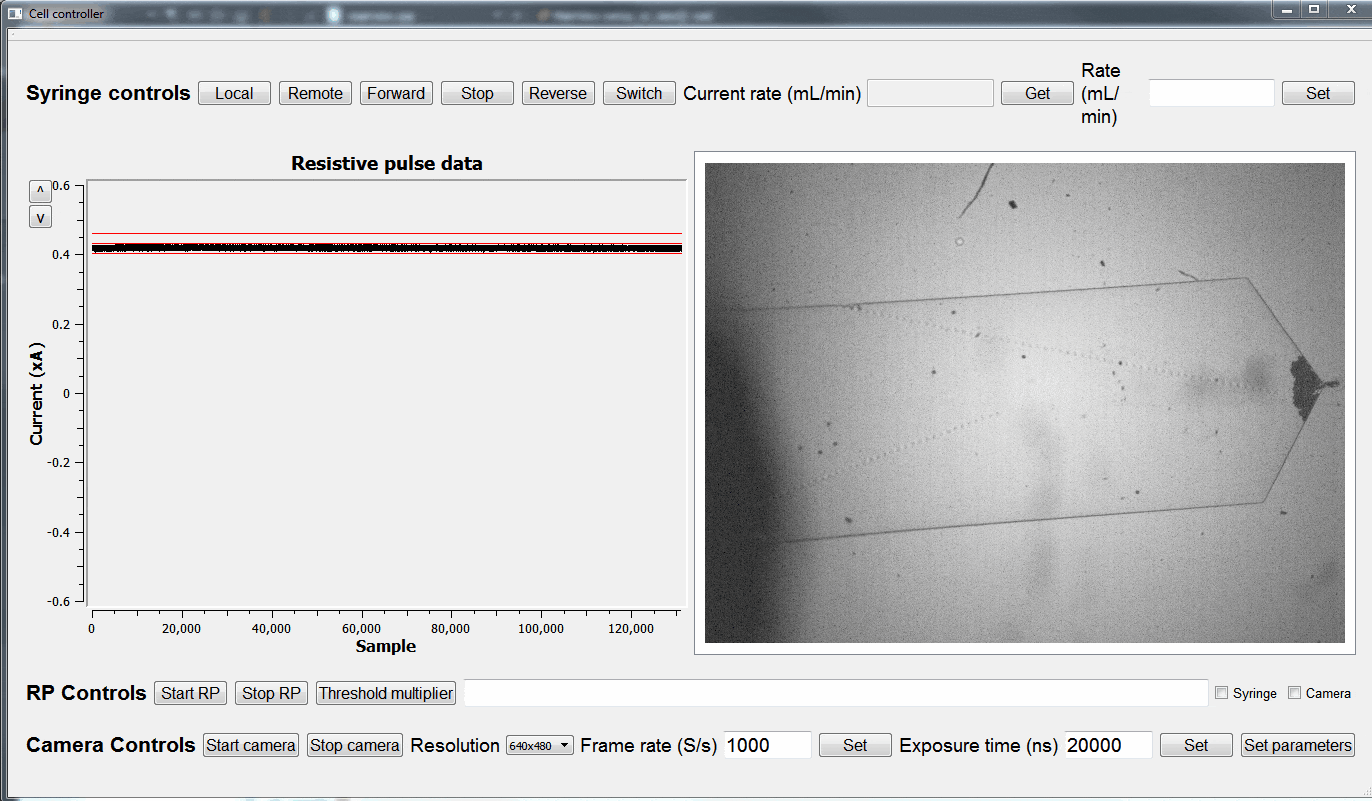
\includegraphics[width=0.5\textwidth]{cellcontroller.png}
			\caption{\textbf{\textit{cell\_controller}, a GUI program written in C++ and the Qt Framework}. The program controls the instruments used to run the experiment.}
			\label{fig:cellcontroller}
		\end{figure}

		
		
		
		
		
		The program used to control each of the instruments used in the experiment was written in C++ and makes use of the Qt framework to provide a GUI environment in which to run the experiment. The program is open-sourced and available at https://github.com/tphinkle/cell\_controller. The software controls the high-speed camera, a data acquisition (DAQ) card used to record the current measurements, and the syringe pump. Each instrument uses its own communication protocol; the high-speed camera is controlled by commands sent via TCP/IP protocol over a 1 GB/s ethernet line, the DAQ card is controlled using the National Instruments NIDAQmx API, and lastly, the syringe pump is controlled via serial commands sent over an RS-232 line. A screen shot of the program is shown in Fig. \ref{fig:cellcontroller}.
		
		
		\begin{figure}[t!]
			\centering
			\begin{subfigure}[t]{0.3\textwidth}
				\centering
				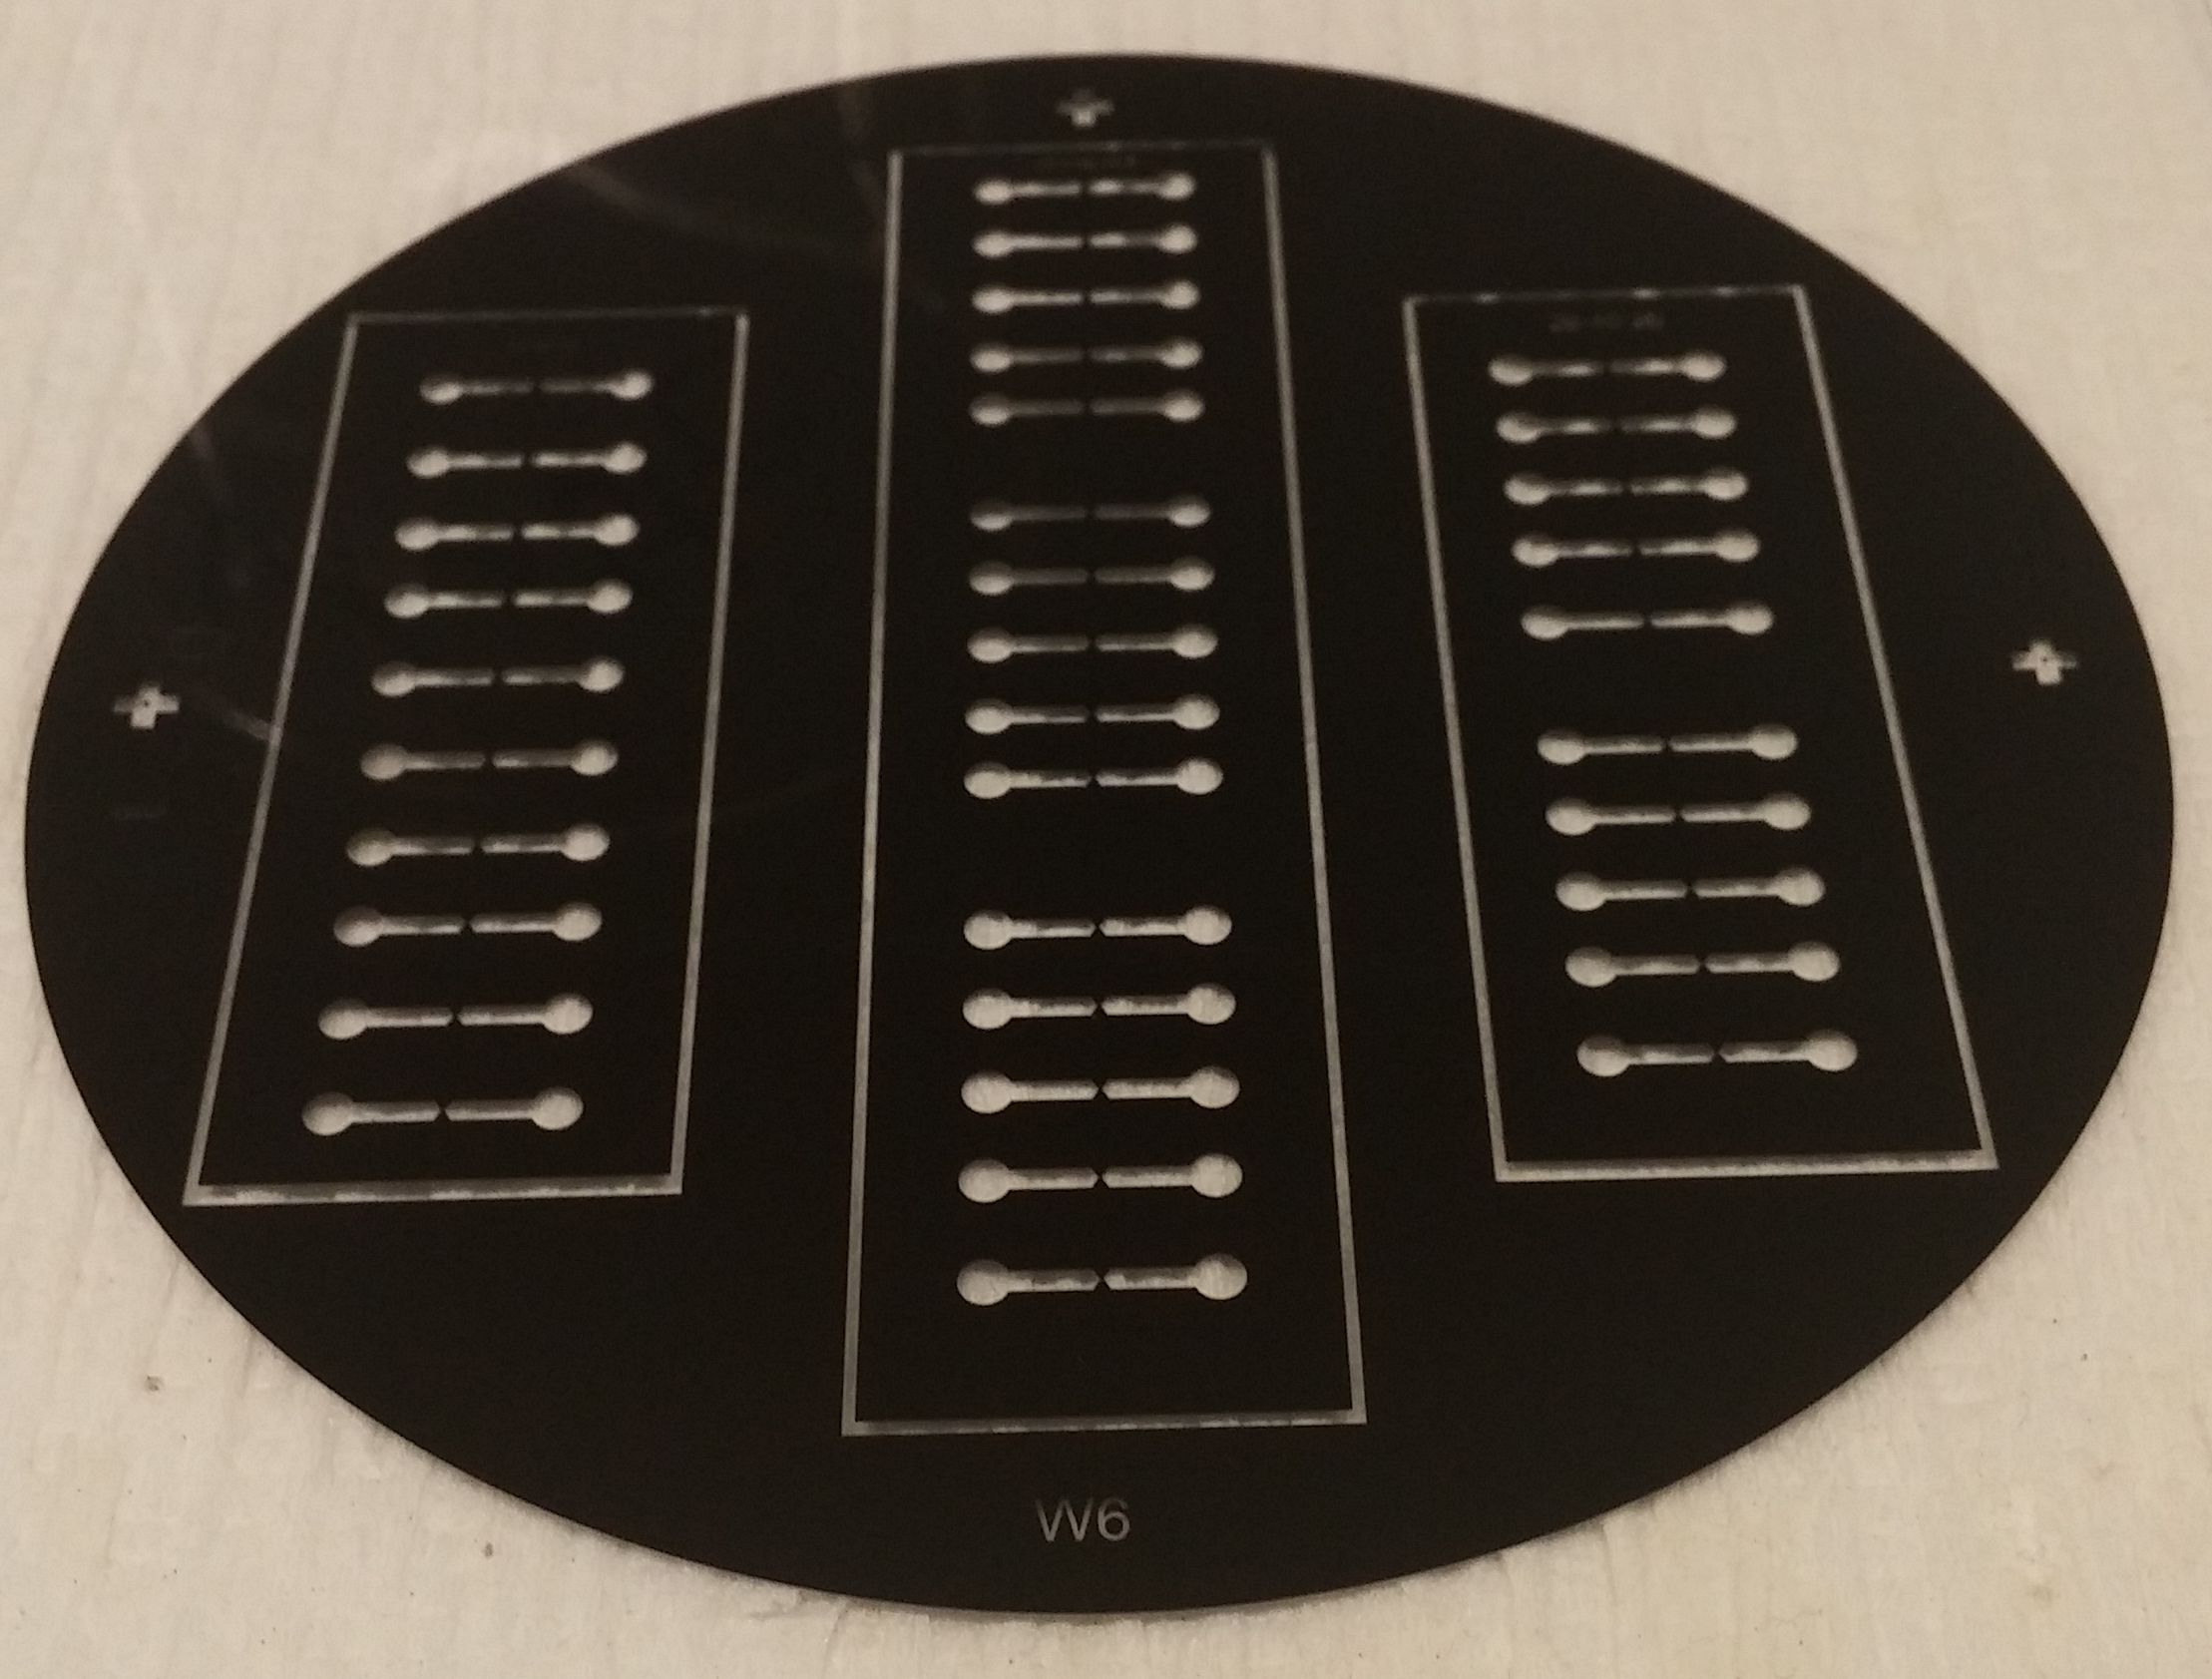
\includegraphics[width=1in]{transparency}
				\caption{\textbf{Printed phototransparency of microfluidic channel designs.}}
			\end{subfigure}
			\begin{subfigure}[t]{0.3\textwidth}
				\centering
				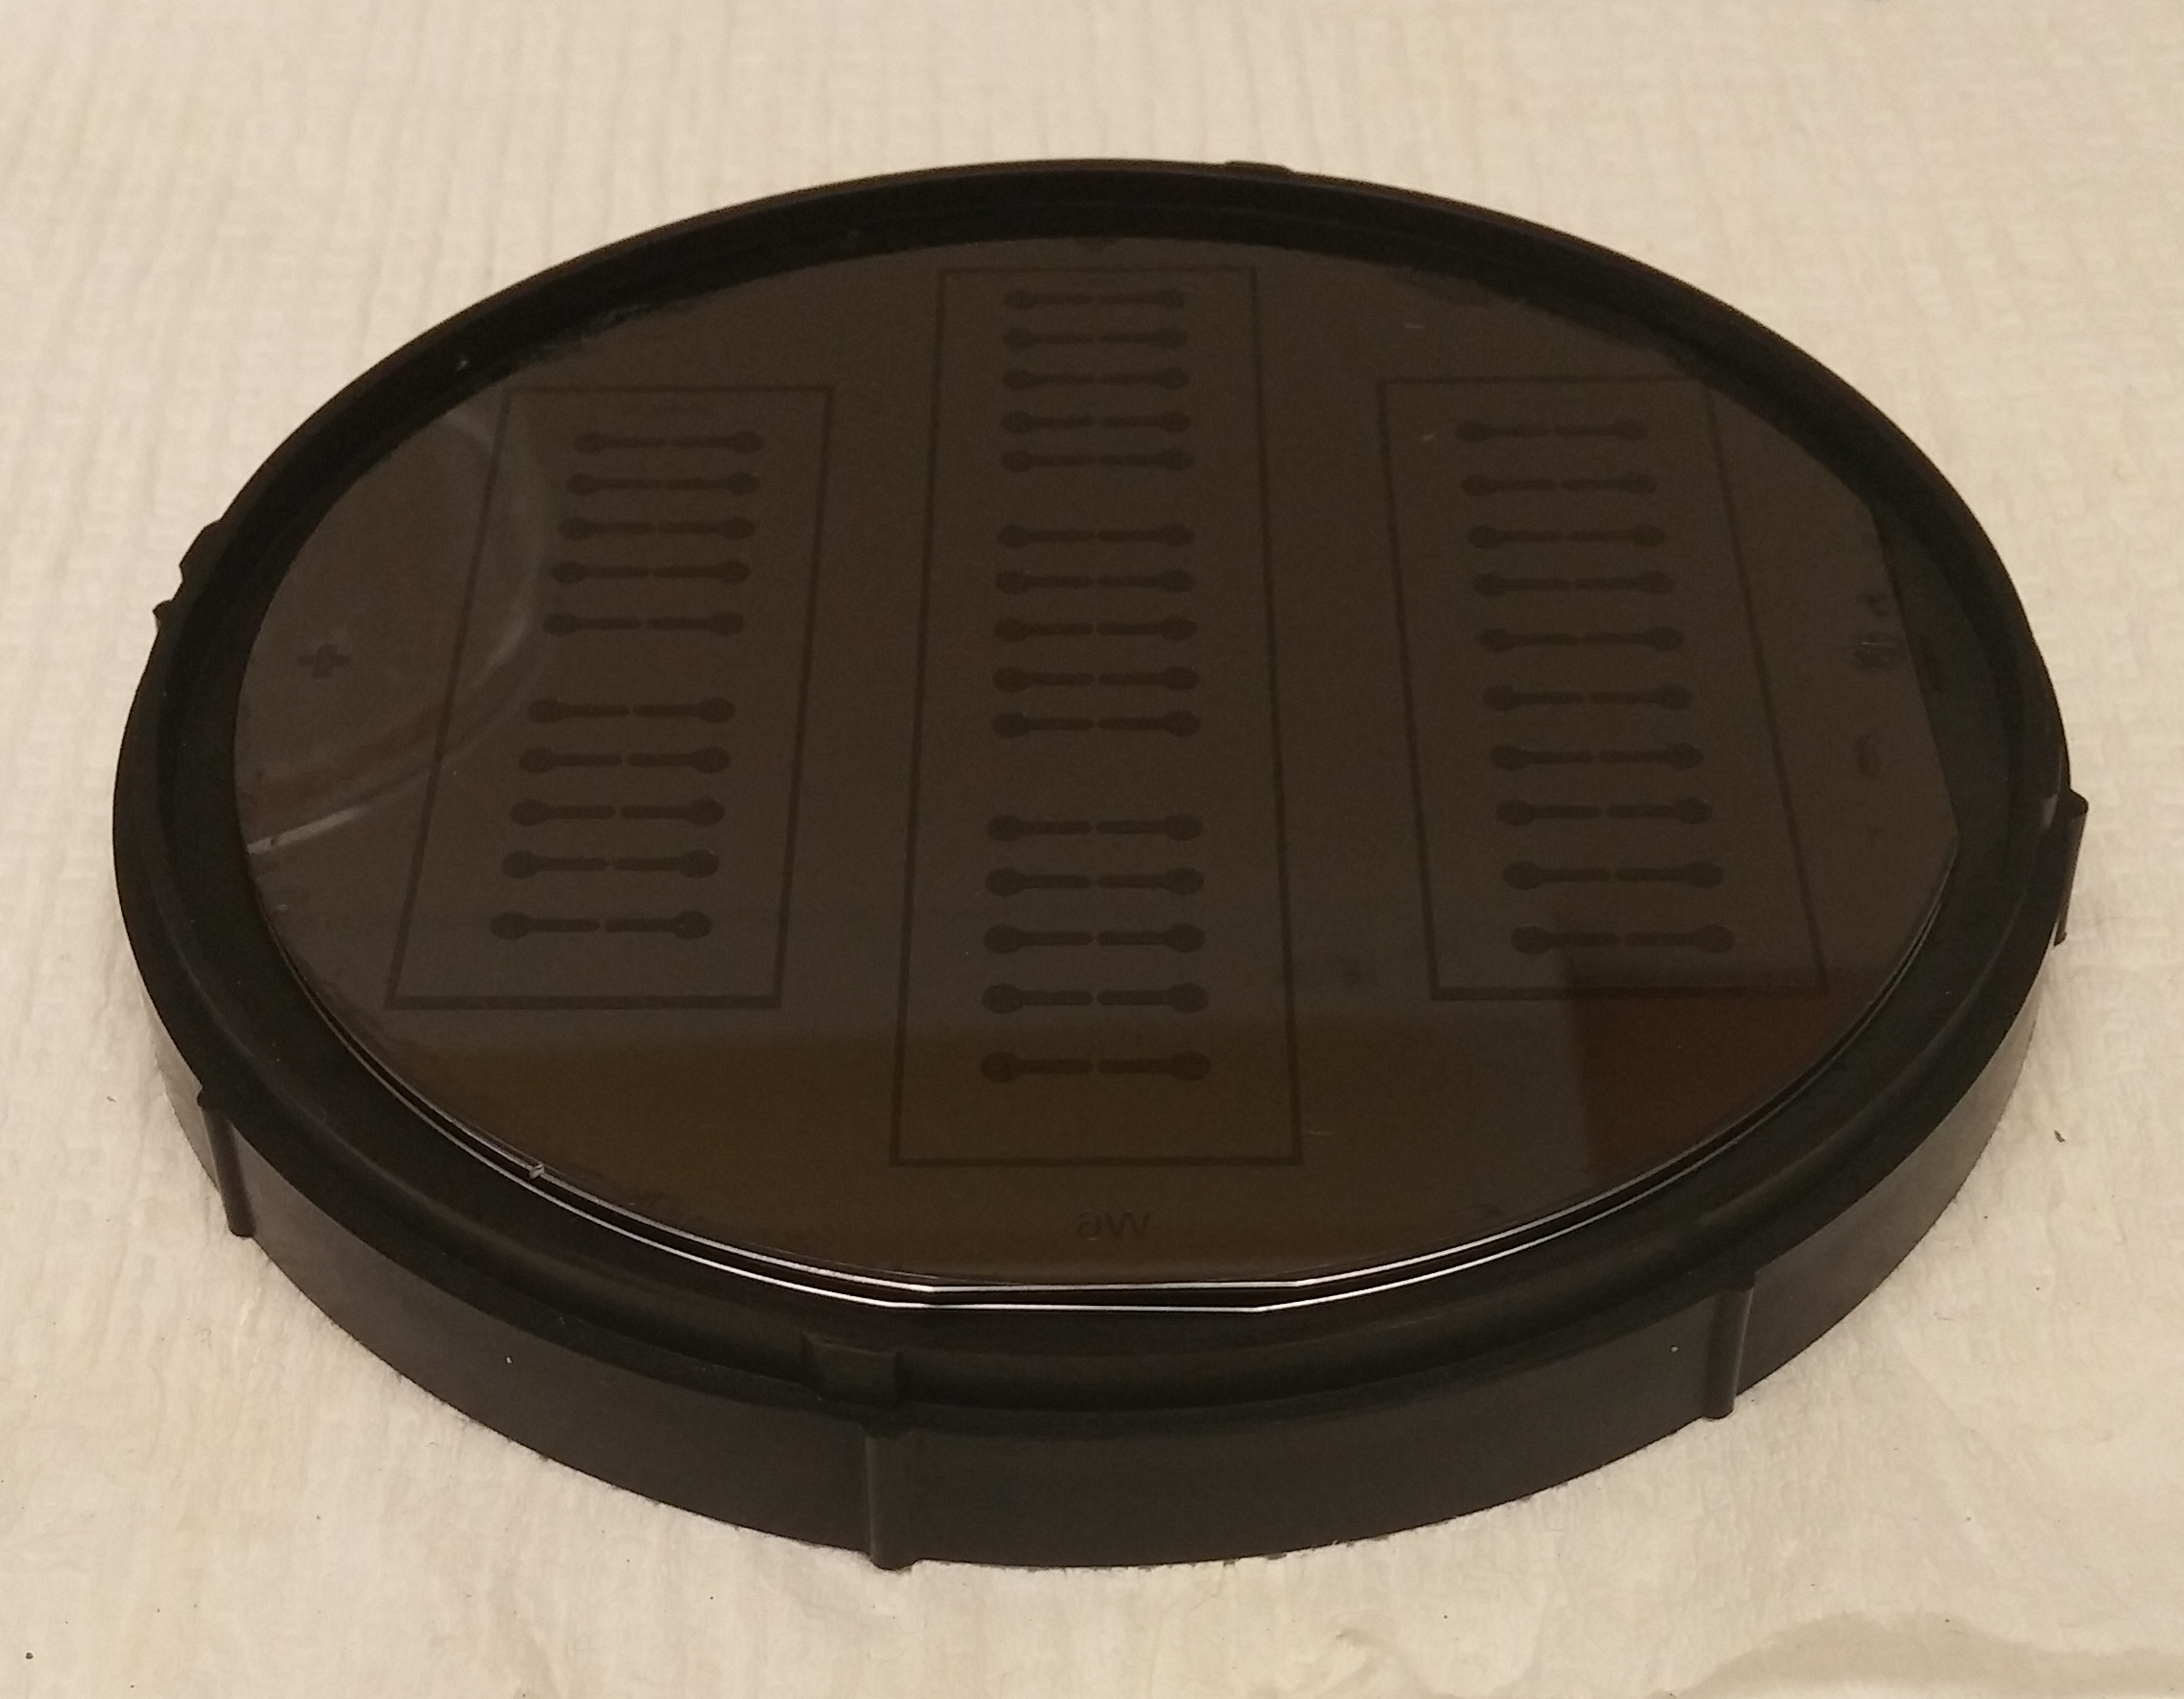
\includegraphics[width=1in]{wafer}
				\caption{\textbf{Channel mold patterned on SU8 photoresist, on a silicon wafer.} The transparency image is patterned onto the SU8 using soft photolithography techniques.}
			\end{subfigure}
			\begin{subfigure}[t]{0.3\textwidth}
				\centering
				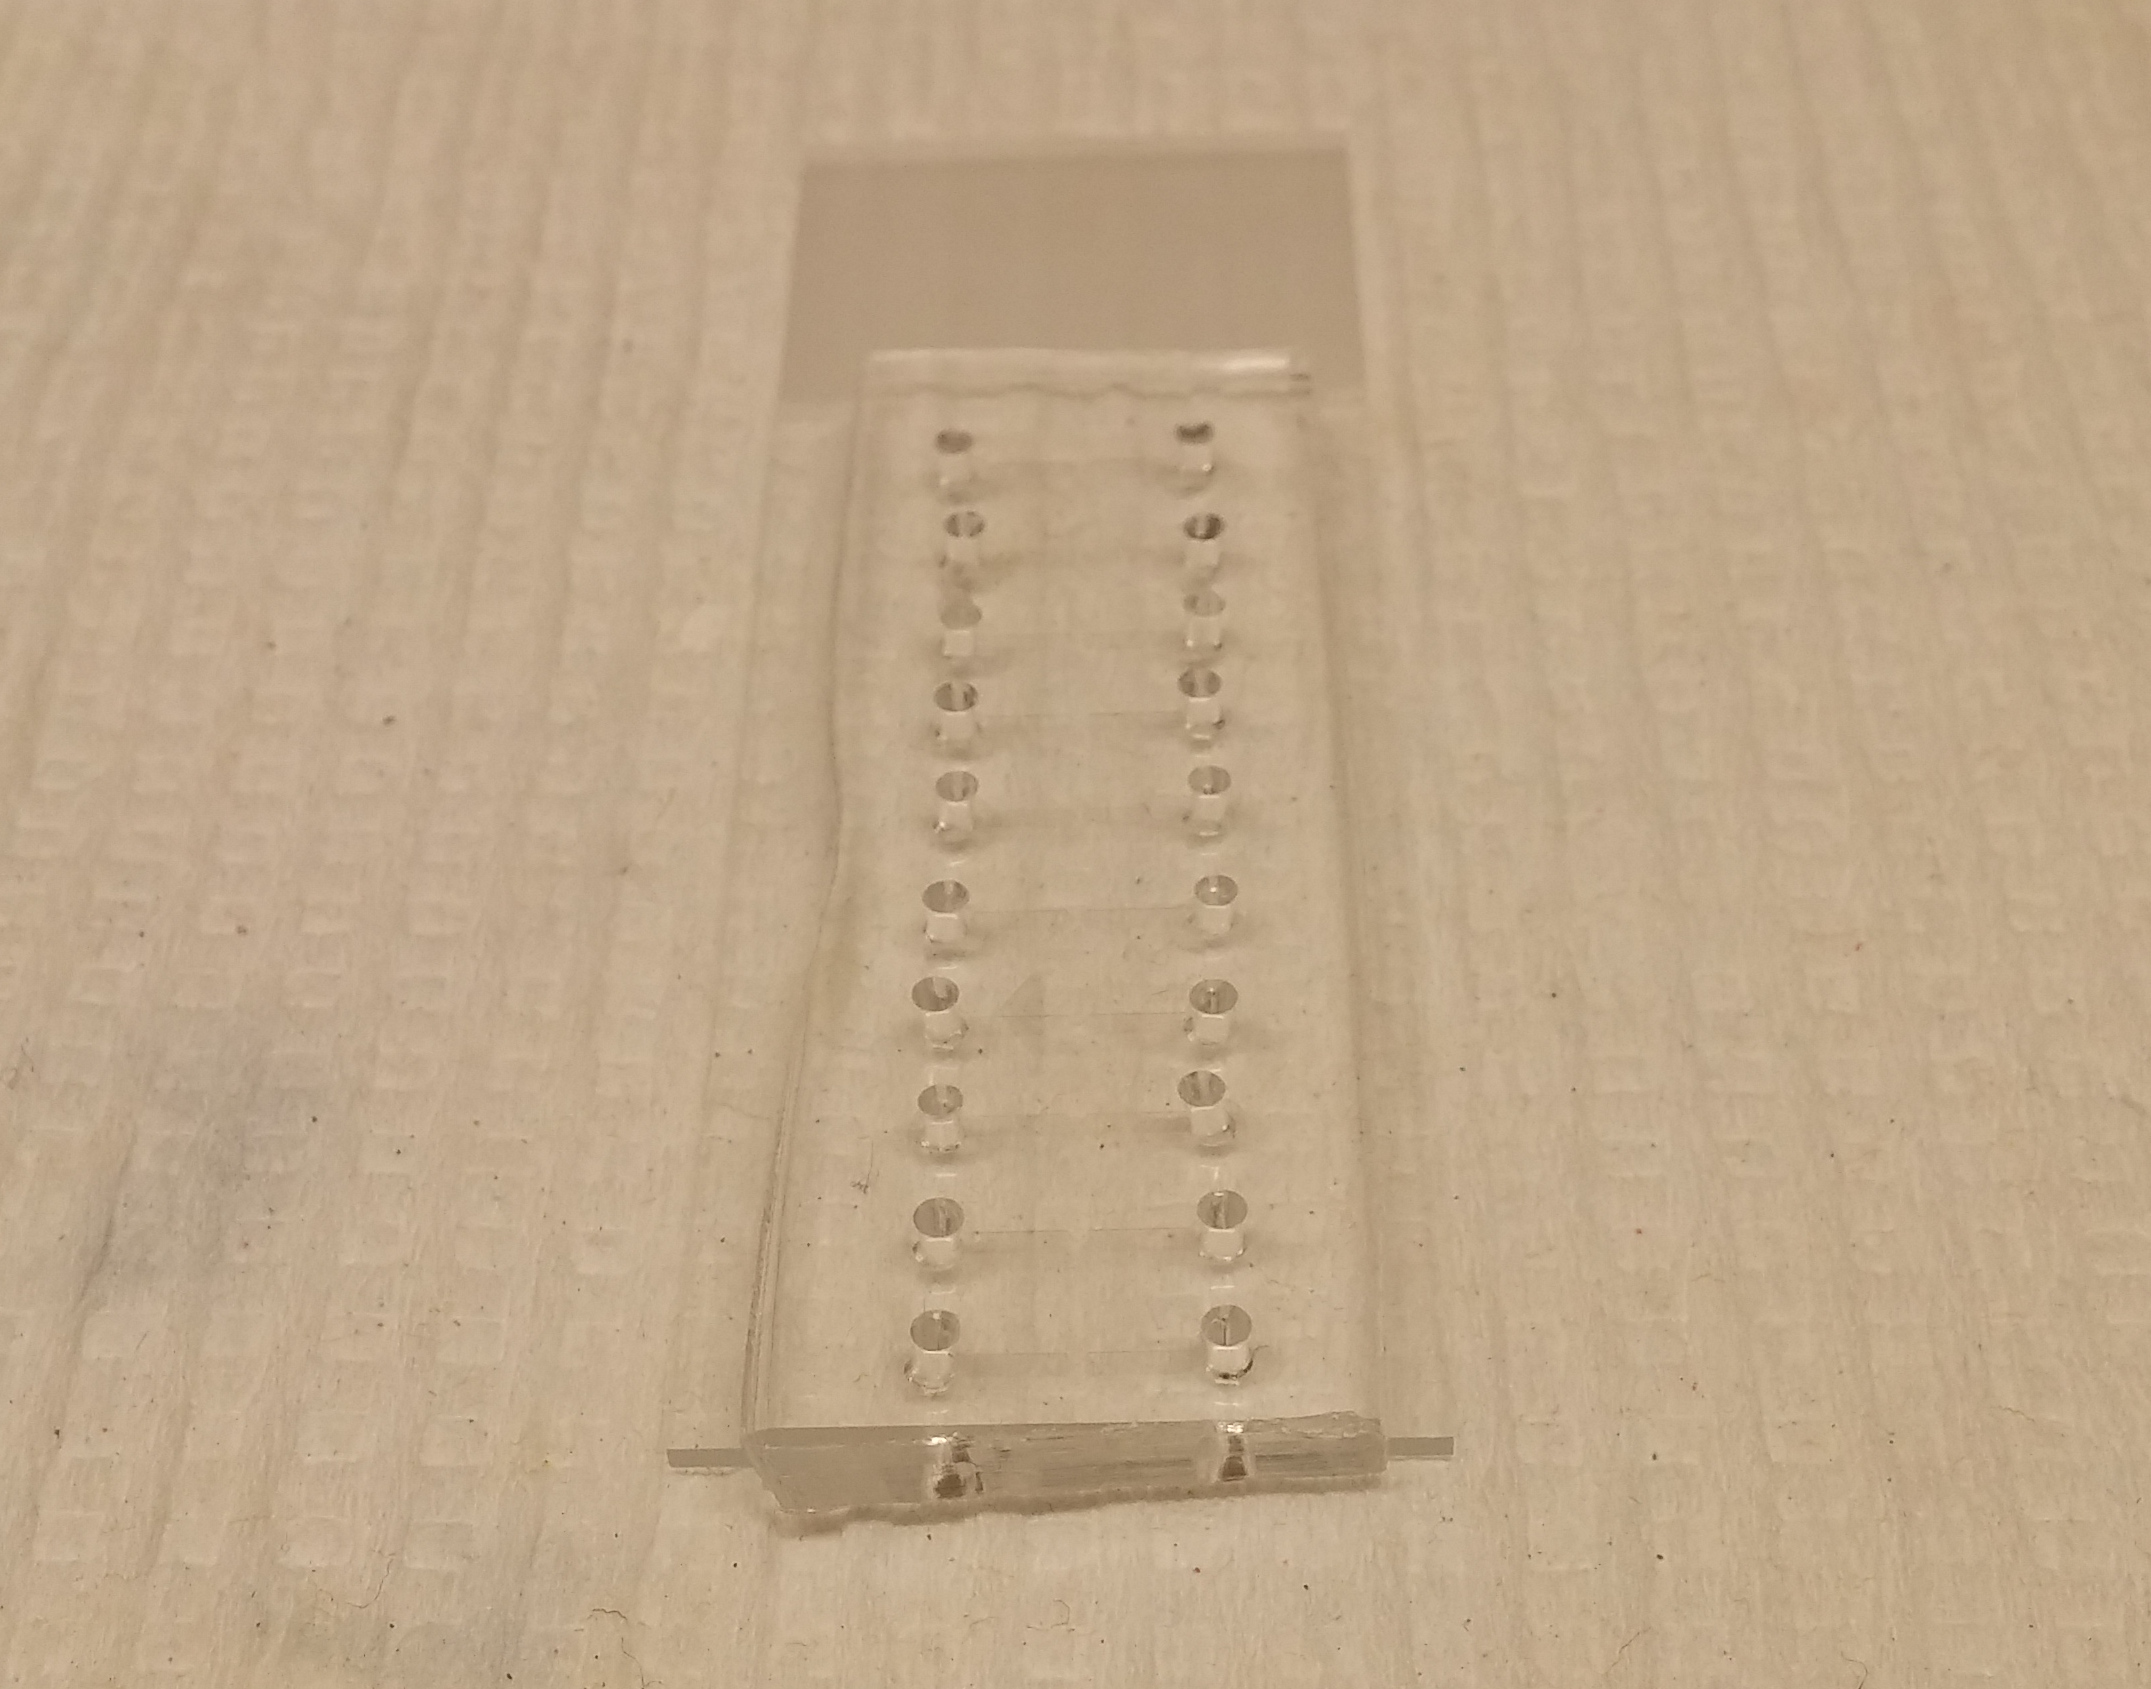
\includegraphics[width=1in]{chip}
				\caption{\textbf{Final PDMS and glass device configuration.} The glass was bonded with the PDMS channels after both were treated in an oxygen plasma. Each row of holes corresponds to a single channel. The holes themselves are the fluid inlet and outlet ports.}
			\end{subfigure}
			\caption{\textbf{Key ingredients in the microfluidic channel fabrication process.}}
		\end{figure}
		
		
		The channels used for these experiments were made from PDMS bonded to a glass slide. PDMS is a transparent elastomer that is relatively inert, transparent, and durable, and for these reasons is probably the most common material used in microfluidic experiments today. Two classes of channels were created in PDMS, constant-width and variable-width, which will be discussed separately in the discussion section. Within each class of channels, different geometries were considered. Images of some of the channels used in the experiments are shown in Fig. \ref{fig:trajectories}, along with lines indicating the tracked trajectories of individual particles (discussed below). $\SI{5}{\mu m}$ polystyrene beads were used as the experimental particle to track, and were suspended in $\SI{1}{M}$ unbuffered KCl solution. The high concentration of solution was chosen because it increases the signal-to-noise ratio, and facilitates analysis of the RP events. The syringe pump rate was chosen to be $\SI{0.005}{mL/min}$, which enabled a large number of events to be detected while also allowing for good sampling of individual events in both the RP ($\SI{250,000}{kHz}$) and IM ($\SI{50,000}{kHz}$ sample, $\SI{10}{\mu s}$ exposure) signals. At this flow rate, particles traveled a small ($\SI{<10}{\mu m}$) distance in between frames, and minimal blurring occured. The \textit{cell\_controller} program recorded the camera and resistive pulse data simultaneously so that the two data streams are guaranteed to capture the same particle translocations.
		
	\section{Data analysis software}
		
		\begin{figure}
			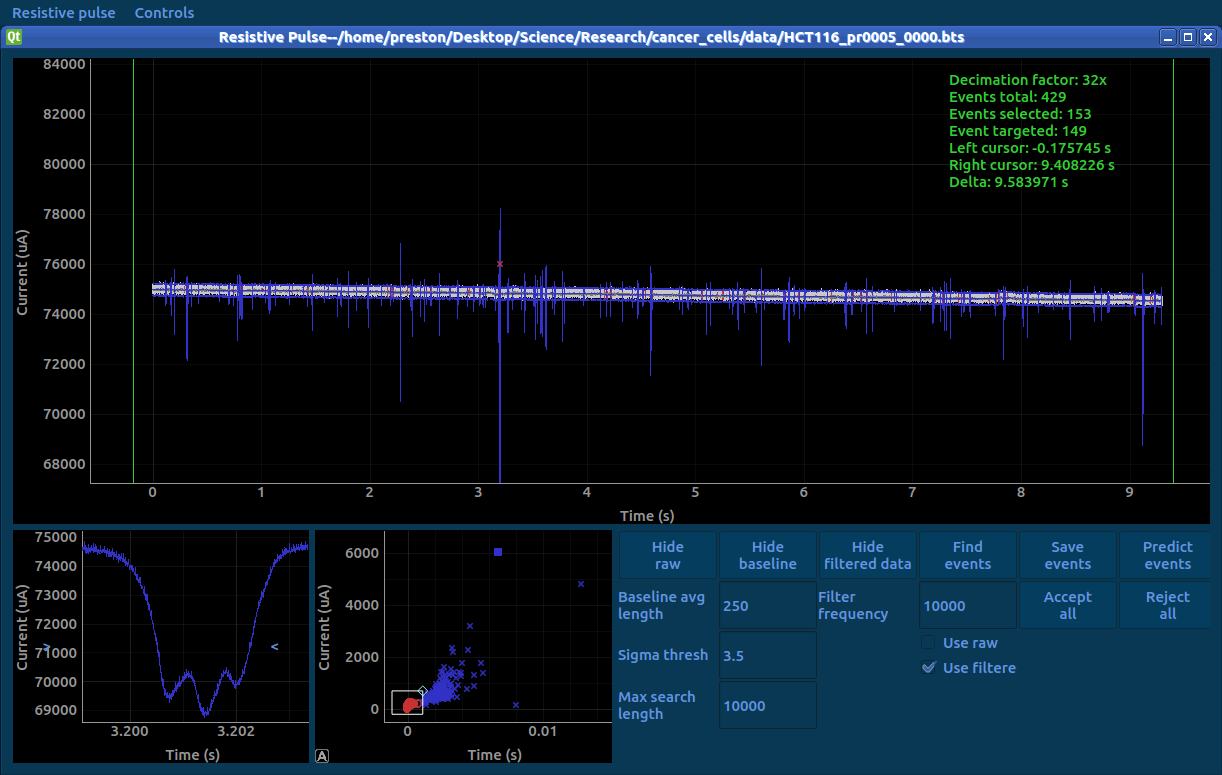
\includegraphics[width=\textwidth]{porestats}
			\caption{\textit{Screen capture of the GUI component of the \textit{pore\_stats} software library.} The program enables fast and accurate extraction of RP events from the baseline data. The main panel shows the raw time-series data (zoomed out), with events that were detected with the program highlighted in blue. The bottom left plot shows a single event that has been targeted by the user. The bottom right plot shows a scatterplot of the current and duration for all events detected, and shows how bulk events can be rejected by selecting a region of the scatter plot. The bottom right buttons and fields are used to change the search parameters, to begin the search, filter data, and enable various other functionalities.}
			\label{fig:porestats}
		\end{figure}

		
		A software library called \textit{pore\_stats} was written in Python and PyQt to facilitate analysis of the resistive pulse data. The program includes a GUI application that can be used to quickly isolate the resistive pulses from the entire time-series. The application includes a number of convenient aspects, including the ability to find events in a drifting or unsteady baseline, the ability to low-pass filter the data to find events with a low signal-to-noise ratio, the ability to filter events based on their amplitude and duration, and a function that allows the user to train a logistic regression model in order to make automatic future accept/reject predictions. A screenshot of the program is shown in Fig. \ref{fig:porestats}. Aside from the GUI program, \textit{pore\_stats} contains a wide variety of functions contained in a library that can be called to perform operations on the RP data, such as filtering, minimum/maximum detection, etc., and to calculate the relevant RP parameters such as duration, amplitude, sub-amplitudes, number of events, event velocity, etc. Finally, because the experiments used for this project include simultaneous resistive pulse and optical tracking, the \textit{pore\_stats} library contains modules for analyzing the imaging data. The library enables detection of particles in individual frames, tracking of particles across frames, and a host of image processing tools that allow the user to calculate physical parameters of interest, such as particle size, aspect ratio, position, etc.
		
	\section{Results \& Discussion}
		
		\subsection{Data analysis explanation}
		
		The experimental hardware and software, and the data analysis software described above were used to perform the experiments and analyze them completely. The data analysis pipeline is as follows. First, the resistive pulse data was opened using the GUI application within the \textit{pore\_stats} library, which was used to extract the detected RP events. Once RP events were detected in the baseline of the time-series, they were saved separately. Next, the camera images were analyzed in order to track optical events. Particles were detected within individual frames using a thresholding approach; a frame in which no particles were present was used as a template, which was subtracted off individual frames. This subtraction yields an image where the pixels of the particles are highlighted white, and everything else is black. A flood-fill algorithm was then used to find incidences of connected pixels, which correspond to individual particle detections. Then, this analysis was performed on hte next image in the camera's recorded video, and particles detected in this frame are connected with particles in the previous frame using a minimum-distance approach. Because we know the exact geometry of the channel, we are also able to determine the physical length of a pixel in the camera image. This is useful because we can then measure distance in physical units (e.g. microns) instead of pixel units. Additionally, we can also use the lines of the channel to create a coordinate system with axes aligned with the axial and lateral directions of the channel. The end result is that through the coordinate transformation and particle tracking, we are able to calculate the actual trajectory in physical units that a particle undertakes when passing through a channel. The trajectory is then described by a sequence of pairs $x_{c}, y_{c}$, where $x_{c}$ are the axial and $y_{c}$ transverse coordinates of the particle with respect to the channel's coordinate frame, in physical units of microns. We chose a coordinate system such that $x_{c}=0$ corresponds to the particle crossing the channel's threshold, and $y_{c}=0$ on the channel's axis.
		
		\begin{figure}
			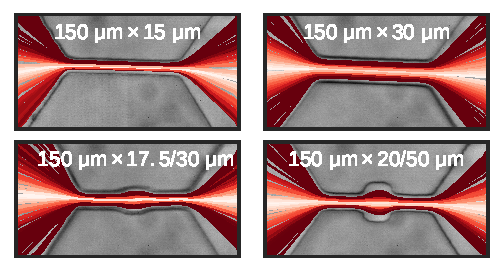
\includegraphics[width=\textwidth]{trajectories.pdf}
			\caption{\textbf{Images of some of the channels used in this study with trajectory lines overlaid.} Each line corresponds to the passage of a single particle through the channel, tracked using image detection techniques. The channels fall into two categories, channels that are complete straight and channels which have central cavities.}
			\label{fig:trajectories}
		\end{figure}

		
		
		Because the particles travel very small distasnces in between frames, tracking individual particles across multiple frames is relatively straight forward. A string of individual detections comprises an IM event. In order to compare the events tracked via RP and IM, a protocol had to be established for matching the events appropriately. In order to do this, we first constructed two time series corresponding to the times of events of the tracked RP and IM signals. The times from one signal ewre shifted until both sequences were seen to overlap. In many cases tracking of some particles fails in either signal. For instance, in the RP signal there could be a brief burst of noise that prevents detection of a pulse in the baseline. In the camera data, failure to track a single particle was less likely to occur, although still possible in principle. Unpaired events were dropped from the respective sequence to which they belonged. After this coarse alignment, we are left with two sequences $IM$ and $RP$ such that every event $i$ in one signal has a matching event $i$ in the other signal that is known to correspond to the same physical particle translocation. However, in order to compare actual data points in the RP and IM signals, a more fine-tuned alignment must be made. In order to perform this exact matching, we find two data points that are known to correspond to the same instant in time (up to the precision of the slower of hte two instruments' sampling periods). For instance, for a pair of detected events in the RP and IM signals, we find the camera frame where the particle occupies the exact center of the channel, and the middle-most data point in the RP signal; we know that both data points correspond to the same instant in time (again, with precision given by the slower of the two sampling periods). Fine alignment of the two time series for each event is then achieved by adding a ismple time offset to one of the signals, equal to the difference in times of the two corresponding data points. In principle, if the camera and DAQ card sampled at exactly the rates specified by their hardware specifications, and this rate did not change within a single recording, fine alignment of the entire time-series would be possible by simply aligning the RP and IM data of a single particle translocation. However, in practice we find that if we apply this offset for a single particle, the signals become out of sync at a later time, which is due to slight inaccuracies in their reported sampling periods. For this reason, we do not apply a single shift to hte time-series in order to align the entire thing, but apply a unique alignment for every pair of events that we compare.
		
		\begin{figure}
			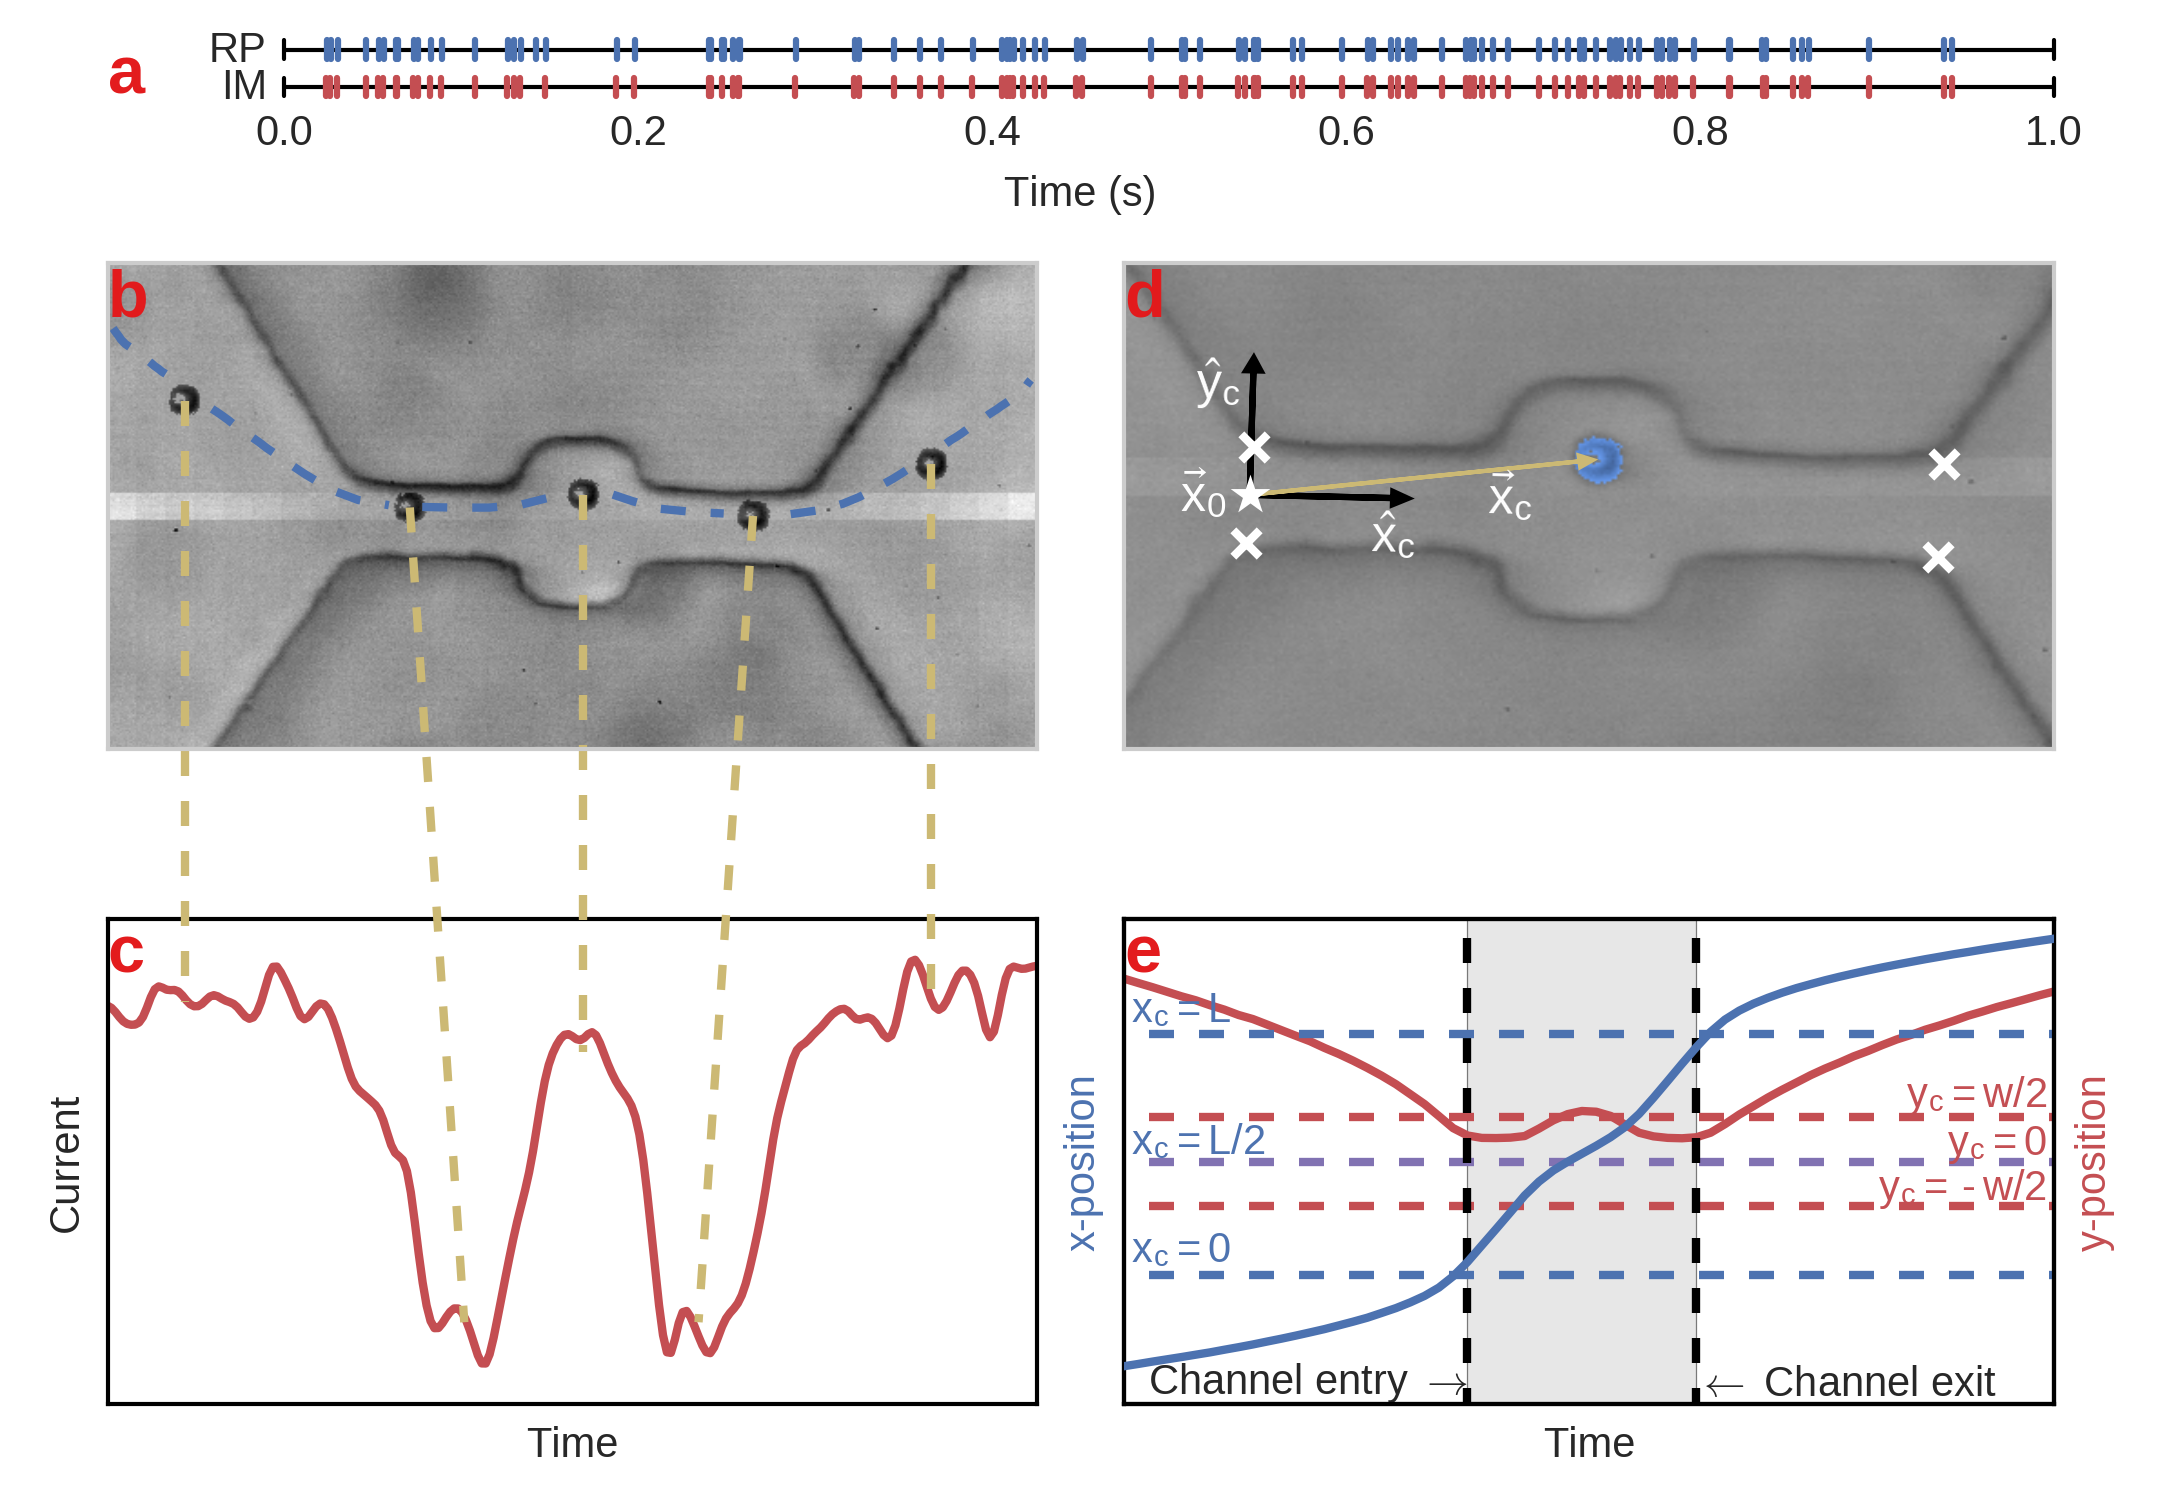
\includegraphics[width=1\textwidth]{rpimsync}
			\caption{\textbf{Event matching protocol for the RP and IM signals.} \textbf{a}.}
			\label{fig:rpimsync}
		\end{figure}

		
		After aligning the two time-series and calculating the position of the particle in the channel's coordinate system, we have a time-series of data $x, y, \Delta I/I_{p}$; in other words, for every event we are able to determine the exact $\Delta I/I_{p}$ for every position in the particle's trajectory through the channel. The event matching protocol, as well as calculation of the particle's positions in the channel's coordinate frame, are shown in Fig. \ref{fig:rpimsync}. 
		

		
		
		
		Armed with the synchronized data set, we can now explore positional dependencies of the RP signals. This matching allowed us to create `resistance maps' of the channel, a picture of the channel that shows the amplitude of the $\Delta I/I_{p}$ at various points. Example resistance maps are shown in Fig. \ref{fig:resistancemaps}. Each data point in the resistance map indicates the position of a single particle at a single point in time, and the color reflects the instantaneous value of $\Delta I/I_{p}$ at that time. In the following sections we analyze resistance maps for straight channels and channels with non-constant widths.
		
		
		\subsection{Straight channels}
		
			\begin{figure}
				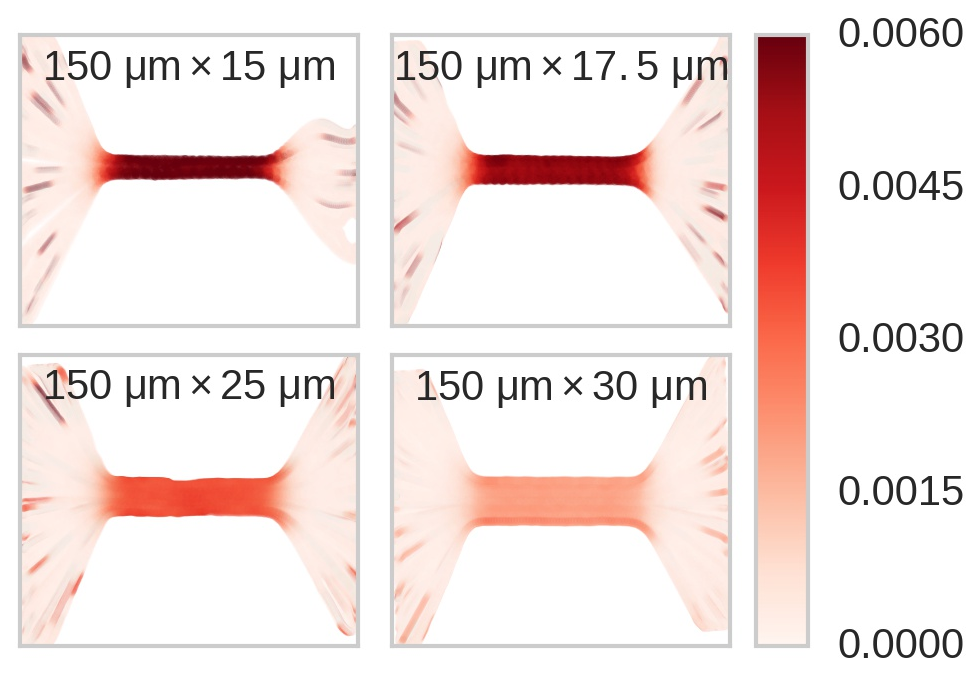
\includegraphics[width=\textwidth]{resistancemaps_straight}
				\caption{\textbf{Resistance maps of the straight channels used in this study.} The resistance maps show that the resistance is most concentrated in the micro constriction, and that the resistance is small elsewhere. A region of finite resistance exists between the micro constriction and the reservoir leading up to the channel. This region is known as the channel's access resistance.}
			\end{figure}

		
			The geometries of the straight channels used in this study are shown in Fig. \ref{fig:trajectories}, top row. The resistance maps determined for these channels are shown in Fig. \ref{fig:resistancemaps_straight}. All channels were approximately $\SI{20}{\mu m}$ in height. The interior regions of hte channels show relativeliy darker red colors than the exteriors, indicating a higher resistance in accordance with our expectations. In the immediate vicinity of the channel, there is a region of moderate resistance known as the access resistance, which extends slightly inside the channel. In the rest of this section we delve into these aspects of the resistance map in greater detail.
			
			
			\subsubsection{Position of maximum RP amplitude in the channel}
			
				\begin{figure}
					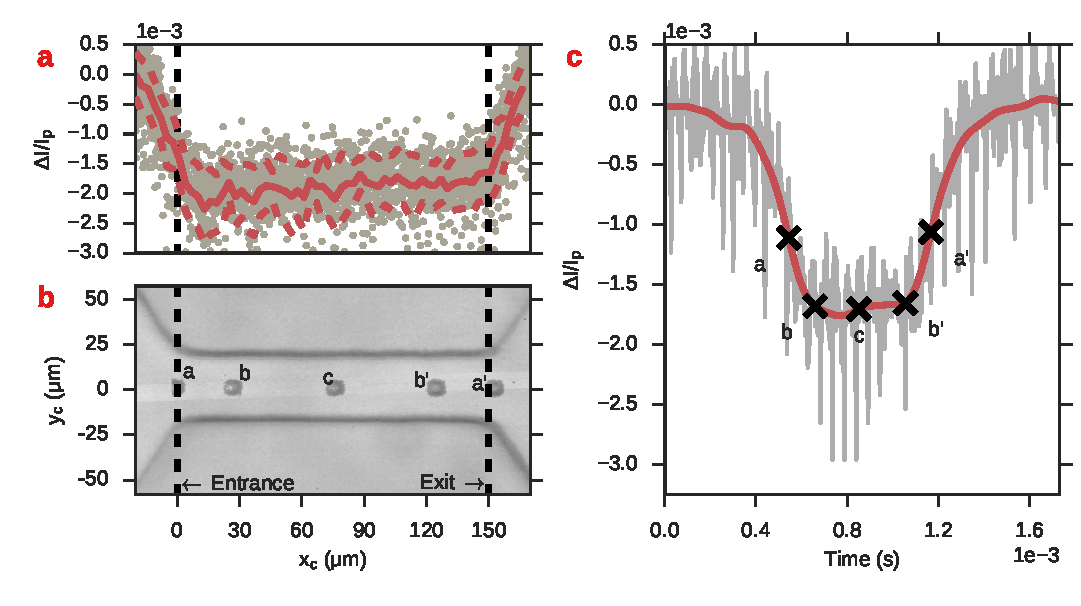
\includegraphics[width=1\textwidth]{channelentrancestraight.pdf}
					\caption{\textbf{Plot of $\Delta I/I_{p}$ vs axial-position $x_{c}$ for polystyrene beads passing through the PDMS channels.} The plots reveal that the current does not reach its maximal value until the particle is well inside the channel.}
					\label{fig:channelentrancestraight}
				\end{figure}

			
				In the traditional RP technique, pulses are usually analyzed for their duration (sometimes called the dwell time) and their amplitude. The pulse duration is a measure of hte particle's velocity, and if the particles are driven through the channel electrophoretically or through electroosmosis, this becomes a basis for measurement of the particle or channel $\zeta$-potential, respectively. However, an exact measurement of the dwell time is always somewhat arbitrary because there is no definitive point in the resistive pulse where we can say the start and stop of the event occurs. Typically some standard is adopted by the researcher for when the beginning and end of an event occur; most researchers choose to use the full-width-at-half-maximum (FWHM) as the points at which the particle enters and exits the channel. The resistance map will allow us to directly observe the current value at the entrance and exits of the channel, and to compare this with the FWHM of the signal to see if this standard is justified. We created plots of hte axial position $x_{c}$ and instantaneous current value $\Delta I/I_{p}$ for each event for the straight channels studied. Figure \ref{fig:channelentrancestraight} shows a single event from the recorded RP time series alongside the data of many events plotted in coordinates of $\Delta I/I_{p} x_{c}$. The figure reveals two interesting features. First, the current does not plateau until the particle is well within the channel, even more than its full diameter. This result is unusual, and suggests that the entrance of the pore has less resistance than its entrance points, even though these points have the same width. Another result is that the point at which the particle crosses the threshold of the channel corresponds very closely to the FWHM of the pulse, a result which suggests that for the purposes of measuring hte dwell time of the particle, the FWHM may be a more accurate estimate than a thresholding approach.
				
				
			\subsubsection{Dependence of resistive pulse amplitude on lateral displacement}
			
				As mentioned in the introduction to this chapter, off-axis translocation of a particle is expected to significantly effect the amplitude of the RP signal it creates. This effect is significant in sizing applications, where it broadens and shifts the distribution of the particles sizes as measured by RP. In order to better understand the effect of off-axis translocation on the RP amplitude, Berge \emph{et al.} performed experiments with particles driven through pores by an induced pressure. As opposed to electroosmosis, pressure-driven flow results in a Poiseuille distribution of the fluid flow rate, which is parabolic and greatly varies across the face of the channel. The experimenters used their knowledge of Poiseuille flow to determine the lateral offset position $y_{c}$ of the particles based on their translocation time. They observed that the slower moving particles with greater offset position also had larger resistive pulse amplitudes than faster moving, on-axis particles. They devised an empirical relationship from the data of the following form:
				
				\begin{equation} \label{eq:berge}
					\frac{\Delta V}{\Delta V_{0}}=1+\alpha\left(\frac{y_{c} d}{D}\right)^{3},
				\end{equation}
				
				where $d$ is the diameter of the particle, $D$ the diameter of the pore, and $\alpha$ was a constant determined to be between $5-7.5$. The equation shows that the distribution of diameters $D$ as determined by RP is both broadened and shifted towards higher diameters by the off-axis effect. Figure \ref{fig:simulateddV} shows simulated data of particles passing through a pore and the resultant measured $\Delta V/V_{0}$ (the quantity measured by Berge in his original work).
				
				\begin{figure}
					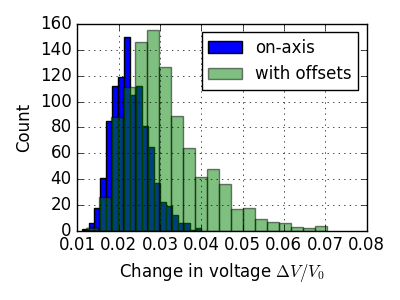
\includegraphics[width=.5\textwidth]{simulated_dV.png}
					\caption{\textbf{Plot of the measured voltage (similar to current) of simulated particle translocations through a pore, with off-axis contribution according to the results of Berge \emph{et al.} (Eq. \ref{eq:berge}).} The plot reveals the effects of off-axis translocation, namely that the distribution of measured $\Delta V$ shifts towards greater values and broadens.}
					\label{fig:simulateddV}
				\end{figure}
				
				
				
				

				
				\begin{figure}
					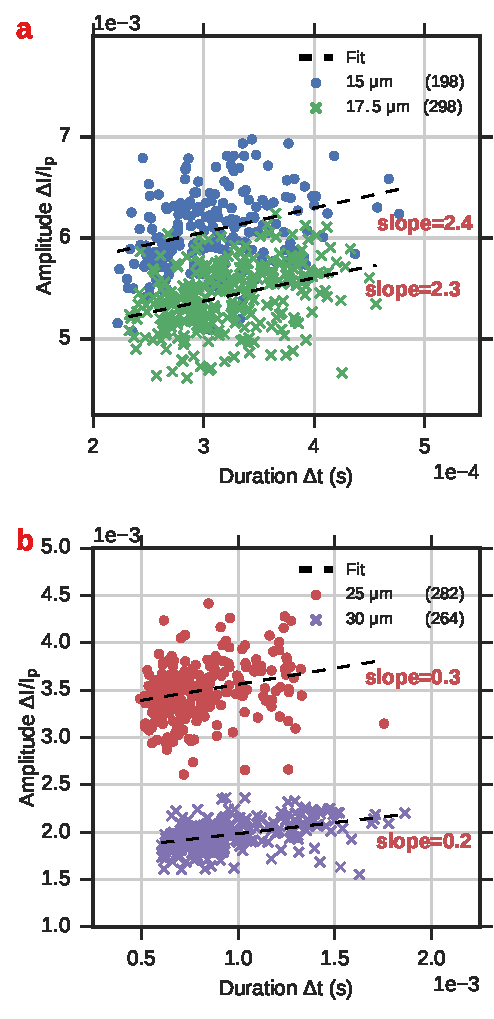
\includegraphics[width=.5\textwidth]{dIdtstraight.pdf}
					\caption{\textbf{Scatter plot of translocation duration $\Delta t$ versus event amplitude $\Delta I/I_{p}$ for the four straight channels studied, with straight line fits.} The fits reveal the positive correlation between translocation time and off-axis position, as observed by Berge \emph{et al.}.}
					\label{fig:dIdtstraight}
				\end{figure}

				
				Although the effect was well-established by the authors, it was only indirectly inferred from the data. Using the hybrid RP-IM approach, we can directly measure the effect of off-axis translocations in RP experiments. Before directly showing the relationship, we first confirmed that we observed the exact same relationship observed by Berge \emph{et al}, namely a positive correlation between translocation time and pulse amplitude. This relationship is shown in Fig. \ref{fig:dIdtstraight}. The scatter data were fit with straight lines, and reveal that not only does the event amplitude increase with increasing translocation time, but that this effect decreases with increasing channel width in accordance with Eq. \ref{eq:berge}.
				
				\begin{figure}
					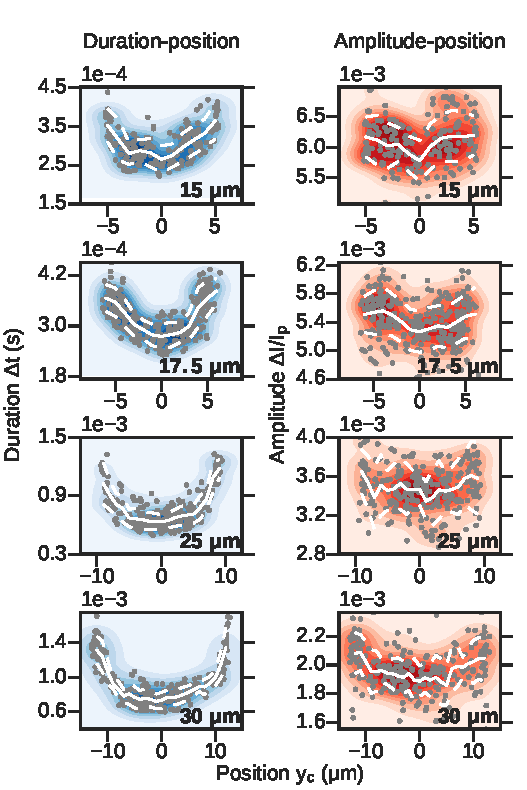
\includegraphics[width=.75\textwidth]{dtdIystraight.pdf}
					\caption{\textbf{Translocation duration $\Delta t$ and RP amplitude $\Delta I/I_{p}$ versus lateral position $y_{c}$ for four straight channels.}}
					\label{fig:dtdIy}
				\end{figure}
				
				The results are shown in Fig. \ref{fig:dtdIy}. The left column of Fig. \ref{fig:dtdIy} shows the translocation time $\Delta t$ versus the off-axis position $y_{c}$ for the straight channels studied, while the right hand column shows $\Delta I/I_{p}$ versus $y_{c}$ for the same events. The left column indicates that the translocation time strongly increases at off-axis positions closer to the channel walls, in accordance with our expectations for the fluid flow profile of Poiseuille flow. Additionally, the right hand figures reveal that the amplitude increase $\Delta I/I_{p}$ also increases for particles passing closer to the channel walls, in agreement with the results observed by Berge \cite{Berge1990} and predicted by Smythe \cite{Smythe1972}. The relationship between amplitude and position is not as strong as of that between translocation time and position, but in all four channels studied we still observed the same dependence. The difference between minimum and maximum $\Delta I/I_{p}$ from the four channels is approximately $8\%$; this difference, while small, is non-negligible and is in rough agreement with the level of difference found in the Berge papers ($10\%$). We note that measurement of the current amplitude of a single event is itself an inherently noisey process. First, the baseline must be accurately determined, which is often an ambiguous measurement, especially when dealing with noisey baseline signals. Second, the interevent current itself is a noisy measurement due to the noise within the signal and the fact that the current level may slightly change during translocation due to non-perfect smoothness of the PDMS channels. For instance, in Fig. \ref{fig:channelentrancestraight}, we see that the event is not perfectly flat, indicating perhaps that there is a small slope in the height of the channel. However, regardless of the noise in the measurement, each of the channels still directly reveal the trend of off-axis translocation increasing the measured resistive pulse amplitude.
				
				
				
		\subsection{Channels with a central cavity}
		
			\begin{figure}
				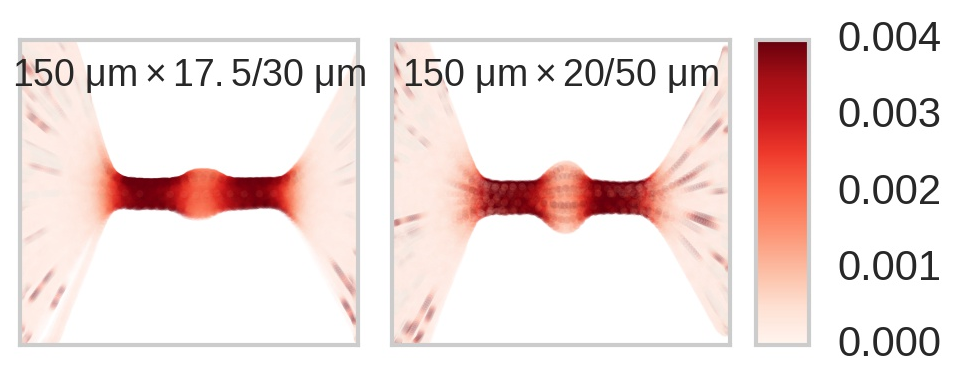
\includegraphics[width=\textwidth]{resistancemaps_cavity}
				\caption{\textbf{Resistance maps of channels having a central cavity.} The resistance maps show that the resistance is most concentrated in the narrow portions of the channel, and less-so in the central cavities (as expected from $R=\rho\int dz/A\left(z\right)$).}
			\end{figure}

		
			The next section covers channels that have a central cavity. The geometry of the devices is shown in the bottom of Fig. \ref{fig:trajectories}. All channels were approximately $\SI{20}{\mu m}$ tall. Resistance maps are shown in Fig. \ref{fig:resistancemaps_cavity}. The geometry used here is somewhat artificial, and channels having central cavities are not a wide class of channels or pores used in resistive pulse studies. However, channels with non-constant widths, and even with widths that discretely changes from one value to another are not uncommon in resistive pulse applications. For instance, one of the most commonly used biological nanopores is known as $\alpha\mathrm{hemolysin}$, which is characterized by having a narrow half and a wide half. However, the particular geometry of a channel with a central cavity was recently proposed as a platform for creating positionally-dependent hydrodynamic forces that can deform particles in a controlled manner. This channel geometry was promoted as a means of probing the deformability of single human cells, a topic that will be discussed in the next chapter of this dissertation. In the rest of htis section, we discuss the distribution of resistance in the channel as determined by the resistance maps, as well as the effects of off-axis translocation of particles. In particular, we find an interesting relationship between off-axis position and pulse amplitude that behaves opposite to what was found in the previous section on straight channels.
			
			
			\subsubsection{Resistive pulse amplitude in the wide and narrow portions of the channels}
			
			\begin{figure}
				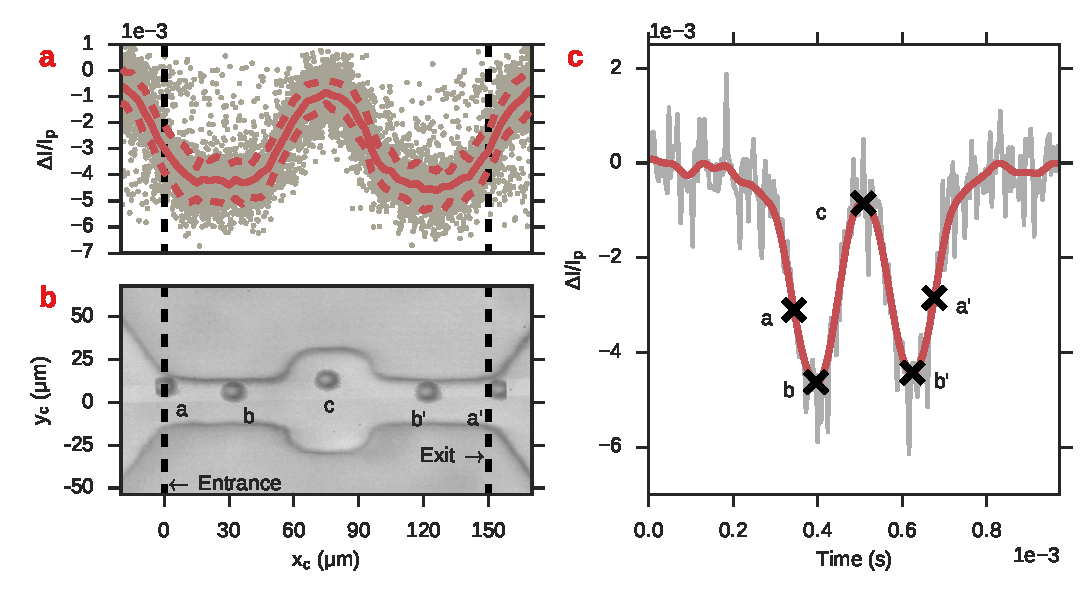
\includegraphics[width=\textwidth]{channelentrancecavity.pdf}
				\caption{Resistive pulse amplitude $\Delta I/I_{p}$ versus axial position $x_{c}$ (a) and versus time $t$ (c). The camera image (\textbf{b}) shows several stills of particle positions aligned with the instantaneous resistive pulse value in the plot above (\textbf{a}).}
				\label{fig:channelentrancecavity}
			\end{figure}

			
			Basic physics considerations suggest that the resistance should be more concentrated in the narrow portions of the channel than in the central cavity, and therefore that the resistive pulse amplitudes hsould be larger in the narrow portions as well. This simple feature of the system is confirmed by the shapes of the individual resistive pulses; an example can be found in Fig. \ref{fig:channelentrancecavity}c. 
			
			\begin{equation} \label{eq:dRlocal}
				\begin{split}
					\Delta R &= \frac{4\rho d^{3}S\left(d/D\right)}{\pi D^{4}} \\
					&= \frac{4\rho d^{3}}{\pi D^{4}}\left[1-0.8\left(\frac{d}{D}\right)^{3}\right]^{-1}
				\end{split}
			\end{equation}

			
			
			However, a more quantitative description of the distribution of the local resistance in the channel is found in equation \ref{eq:dRlocal} \cite{Deblois1977}. Since our experiment measures the current rather than the resistance, we can use our experimental data to verify Eq. \ref{eq:dRlocal} by observing that $\Delta R/R_{0}=\Delta I/I_{p}$, and therefore
			
			\begin{equation} \label{eq:currentratio}
				\frac{\Delta I/I_{p}|_{x_{c}=x_{c1}}}{\Delta I/I_{p}|_{x_{c}=x_{c2}}}=\frac{\Delta R/R_{0}|_{x_{c}=x_{c1}}}{\Delta R/R_{0}|_{x_{c}=x_{c2}}}=\frac{\Delta R|_{x_{c}=x_{c1}}}{\Delta R|_{x_{c}=x_{c2}}}.
			\end{equation}
			
			
			
			\begin{figure}
				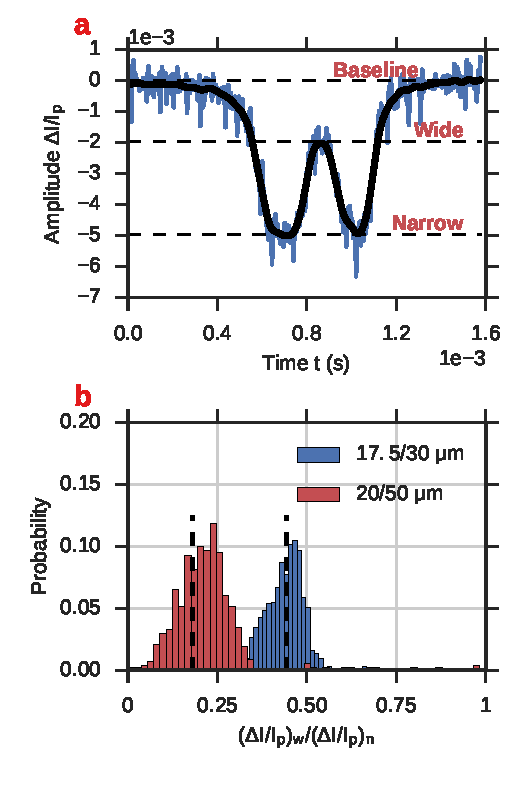
\includegraphics[width=.5\textwidth]{amplituderatios.pdf}
				\caption{\textbf{Histograms of the ratios of the pulse amplitude $\Delta I/I_{p}$ in the narrow portion of the channel and in the central cavity for the two types of cavitated channels studied.} The dashed lines indicate the theoretical values predicted by Eq. \ref{eq:currentratio}. In both cases, the theoretical predictions closely match the experimentally obtained results.}
				\label{fig:amplituderatios}
			\end{figure}

			
			
			
			
			Equation \ref{eq:dRlocal} can be substituted into the final expression in \ref{eq:currentratio}, and therefore the equation allows us a means of comparing the experimentally obtained values for $\Delta I/I_{p}$ with the theoretical equations. This operation was performed for each of teh chanels with central cavities, with $x_{c1}$ corresponding to the particle occupying hte narrow portion of hte channel, and $x_{c2}$ corresponding to the particle occupying the exact middle of the cavitated part of the channel. The results are shown in Fig. \ref{fig:amplituderatios}. The histograms indicate the distribution of the experimentally measured ratios, while the dashed lines represent the theoretical predictions of equation \ref{fig:currentratio}. The spread in each distribution is a combination of measurement error on the exact values of the current, an intrinsic (although small) spread in the distribution of sizes of the particles, and perhaps most importantly, the distribution of off-axis positions $y_{c}$, which we showed significantly contributed to the measured $\Delta I/I_{p}$ in the previous section, and which we will further discuss in the next section. While the dashed lines overlap well with the actual distributions, we note that there is a discrepancy in both cases. Equation \ref{eq:currentratio} was derived for spheres moving through cylindrical channels only, and so we expect that our channels, which have rectangular cross-sections, may not adhere perfectly. In using Eq. \ref{eq:currentratio}, we approximated our channels as cylinders having radii that would yield a cross-sectional area the same as the actual cross-sectional area of the rectangular channels. This approximation will be more accurate for low-aspect ratio cross sections (i.e. squares), and less-so for larger aspect ratio channels. This observation agrees with our findings: the $20-50-20 \mu\mathrm{m}$ channel has a larger aspect ratio in its cavity, and also happens to have a greater discrepancy between the experimental results and the theoretical predictions of Eq. \ref{eq:currentratio}.
			
		\subsubsection{Dependence of resistive pulse amplitude on lateral displacement in narrow and wide (cavity) regions}
		    
			\begin{figure}
				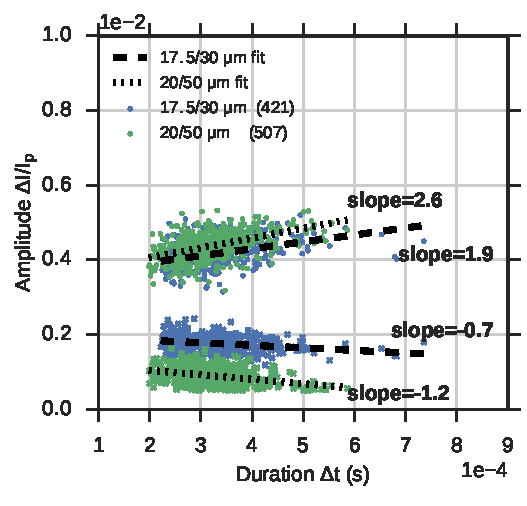
\includegraphics[width=\textwidth]{dIdtcavity.pdf}
				\caption{\textbf{Pulse amplitude $\Delta I/I_{p}$ in the narrow portion and central cavity versus translocation time $\Delta t$ for particles passing through the cavitated channels.} The plots reveal a positive correlation between translocation time and pulse amplitude in the narrow portion of the channel, but a negative correlation between translocation time and the pulse amplitude measured in the central cavity.}
				\label{fig:dIdtcavity}
			\end{figure}

		    
		    
		    
			In the previous section on straight channels, we looked at the dependence of lateral displacement on the measured current amplitude $\Delta I/I_{p}$. In this section, we would like to explore the same relationship but this time for two regions, the narrow constriction and the central cavity. Retracing our footsteps from the previous section, Fig. \ref{fig:dIdtcavity} shows the resistive pulse amplitudes $\Delta I/I_{p}$ versus translocation time $\Delta t$ for particles passing through the channels, but this time including both the pulse amplitude in the central cavity in addition to its value in the narrow constrictions. Interestingly, while the positive correlation observed previously is still observed, we observe a negative correlation between translocation time and pulse amplitude for particles in the cavity. This result suggests that events with longer translocation times, presumably still those translocating close to the walls, will have larger pulse amplitudes in the narrow constriction but smaller pulse amplitudes in the cavities compared to on-axis translocating particles.
			
			\begin{figure}
				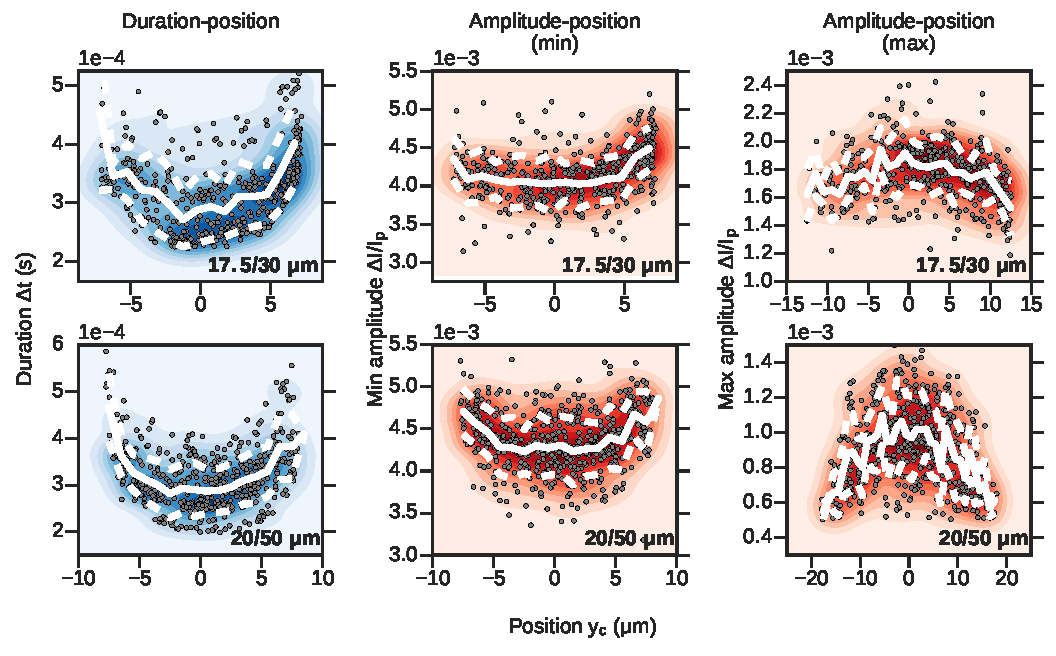
\includegraphics[width=\textwidth]{dtdIycavity.pdf}
				\caption{\textbf{Translocation duration, pulse amplitude in the narrow constriction, and pulse amplitude in the central cavity versus off-axis position for the two channels with central cavities studed in this work.}}
				\label{fig:dtdIycavity}
			\end{figure}

			
			In order to directly confirm the connection between off-axis position $y_{c}$ and pulse amplitude $\Delta I/I_{p}$, we measured the two values instanteously and plotted the results. Figure \ref{fig:dIdtycavity} is analagous to Fig. \ref{fig:dIdtystraight}, but includes positions when the particle is in the narrow portion of the channel and when it occupies the central cavity. Starting with the left column of the figure, we see that particles that translocated near the wall of the cavity had longer translocation times, in accordance with our expectations from Poiseuille flow profiles. In the case of particles having a central cavity, the fluid flow profiles are undoubtedly more complex than a simple Poiseuille flow; however, we expect that the general trend of a central maximum in the fluid velocity and zero fluid velocity at the channel walls will still hold due to basic considerations about non-slip conditions and viscous coupling between laminar sheaths within the fluid. The next column shows the relationship between amplitude and lateral position in the narrow part of the channel. Not surprisingly, the plots show an increase in the current amplitude when particles translocate closer to the walls, in accordance with our findings for completely straight channels. Finally, in the third column we plot current pulse amplitude versus off-axis position while the particle occupies the central cavity. First, notice that the spread in $y_{c}$ is greater than in the cavity. This greater spread reflects the fact that particles translocating close to the wall follow the contours of the channel, and can swing into the cavity during their translocation, having greater off-axis positions than is possible in the narrow portion. The plot reveals a striking difference between the off-axis effect in the narrow and in the wide portions. Instead of increasing the current amplitude, off-axis translocation greatly decreases the current amplitude in the cavity. Furthermore, the decrease in the current amplitude is upwards of $40\%$, a much greater difference than the maximum of $\sim10\%$ observed for the excess of the current amplitude due to off axis translocation in the narrow portion of the channel. This result has great implications for any resistive pulse studies using channels with cavities and or channels with varying widths. To give specific examples, polyethylene terephthalate pores (discussed in \ref{chap:rods}) have natural undulations in their interior diameter that can have cavity-like features. In the next chapter we discuss how the microfluidic channels discussed here may be used with resistive pulse to measure the deformability of cells; in this case, the off-axis translocation effect will be especially significant.

			
		
	\section{Conclusion}
		In this chapter we introduced a hybrid resistive-pulse optical measurement detection platform. The platform may be used to enhance the characterization of single particles by providing new information (features) of their passage. Perhaps most importantly, the platform can be used to validate resistive pulse measurements, which are prone to distortion by effects relating to geometry and position that cannot be verified through the resistive pulse signal alone. Therefore, we suggest the greatest use of this hybrid measurement system will be in validating the measurements of specific resistive pulse platforms.
		
		However, we must point out that the experiments conducted here are necessarily at the microscale, since, as discussed earlier, optical imaging is only possible above the diffraction limit of $\SI{200}{nm}$. Furthermore, we argued earlier that resistive pulse experiments are most widely employed to study particles below the optical diffraction limit. Therefore, at first glance it appears that the results presented here are of no use to resistive pulse experiments. However, the positional effects that distort RP measurements are size independent. To understand why, note that the size effects all originate due to the distortion of the electric field along the boundaries present in the system. In the mean field approximation, the electric field lines are scale invariant--they only depend on the particular geometry of the system. As a concrete example, a $\SI{10}{\mu nm}$ sphere inside a $\SI{20}{\mu m}$ cylindrical channel will experience the same positional effects as a $\SI{10}{nm}$ sphere inside a $\SI{20}{nm}$ cylindrical channel. That is, the overall \textit{scale} of the physics involved does not matter, only the relative sizes of the entities imposing the electrostatic boundary conditions in the problem. Therefore, we expect that the effects studied in this paper generalize down to the sub-micro scale and beyond. However, we can only claim the physics pertaining to the electrostatics of the problem generalize down to the nanoscale. At the nanoscale, a wealth of new physics presents itself, including electrostatic screening at charged surfaces, electroosmosis, and electrophoresis. Therefore, we do not suggest that this paper's results are directly translatable down to the nanoscale, but rather that the results superimpose with the physics native to the nanoscale. Nevertheless, we believe that the results in this work can serve as useful considerations for understanding RP experiments in nanoscale systems, and the general principle of simultaneous RP and IM can be applied to study other important aspects of RP experiments not covered in this work.
		
		
		



%%% Local Variables: ***
%%% mode: latex ***
%%% TeX-master: "thesis.tex" ***
%%% End: ***
